\documentclass[output=paper,colorlinks,citecolor=brown]{langscibook}
\bibliography{localbibliography}

%\author{Mojmír Dočekal\orcid{0000-0002-9993-4756}\affiliation{Masaryk university} }
\author{John Doe}

% replace the above with you and your coauthors
% rules for affiliation: If there's an official English version, use that (find out on the official website of the university); if not, use the original
% orcid doesn't appear printed; it's metainformation used for later indexing

%%% uncomment the following line if you are a single author or all authors have the same affiliation
\SetupAffiliations{mark style=none}

%% in case the running head with authors exceeds one line (which is the case in this example document), use one of the following methods to turn it into a single line; otherwise comment the line below out with % and ignore it
%\lehead{Šimík, Gehrke, Lenertová, Meyer, Szucsich \& Zaleska}
%\lehead{Mojmír Dočekal}
\lehead{John Doe}


\title{Equatives and two theories of negative concord}
% replace the above with your paper title
%%% provide a shorter version of your title in case it doesn't fit a single line in the running head
% in this form: \title[short title]{full title}
\abstract{This article reports the results of an experiment targetting the acceptability of Czech neg-words and strong NPIs under Neg-Raising predicates and in the complement clauses of equatives. The theoretical consequences of the results are discussed and range from the support of non-standard negative concord theories to the support of non-standard degree semantics for the equative constructions. 

\keywords{experimental semantics, Czech, neg-words, strong NPIs, equatives}
}

%%%%%%%%%%%%%%%%%%%%%%%%%%%%%%%%%%%%%%%%%%%%%%%%%%%%
%%%                                              %%%
%%%           PACKAGES                           %%%
%%%                                              %%%
%%%%%%%%%%%%%%%%%%%%%%%%%%%%%%%%%%%%%%%%%%%%%%%%%%%% 

\usepackage{langsci-lgr}
\usepackage{langsci-osl}
\usepackage{langsci-gb4e}
\usepackage{langsci-cgloss}
\usepackage{langsci-affiliations}
\usepackage[linguistics]{forest}
\usepackage{langsci-optional}

% add any extra packages below, but use them only if it's really necessary
\makeatletter
\let\thetitle\@title
\let\theauthor\@author 
\makeatother

\newcommand{\togglepaper}[1][0]{ 
%   \bibliography{../localbibliography}
  \papernote{\scriptsize\normalfont
    \ResolveAffiliations
      [output affiliation=false, output authors font=\normalfont]
      {\theauthor}.
    \titleTemp. 
    To appear in: 
    Change Volume Editor \& in localcommands.tex 
    Change volume title in localcommands.tex
    Berlin: Language Science Press. [preliminary page numbering]
  } 
  \pagenumbering{roman}
  \setcounter{chapter}{#1}
  \addtocounter{chapter}{-1}
}

\newcommand{\orcid}[1]{}

\AtBeginDocument{\nogltOffset} %removes extra spacing before trans line in examples

\togglepaper[42]
% the chapter number will be provided by volume editors; for now keep this way

\begin{document}
\maketitle

\section{Introduction}\label{intro}

In this article, I examine expressions depending on the polarity. The evidence comes from Czech, a strict negative concord language. I will focus on one recent experiment in the paper, but the experiment is a continuation of many previous experimental works which incrementally changed the nature of questions and research goals reflected in the current experiment; see \sectref{sec:acknowl} for the list of people to whom I'm more than happy to thank for their cooperation. The theoretical ambition of this paper is to add to experimental research on Negative Polarity Items (NPIs) like \citet{Chemla-Homer-Rothschild-NPI,gajewski2016another,alexandropoulou2020there} a.o., more specifically to the style of NPI experimental works found in \citet{djarv2018cognitive,schwarz2020italian} and their experimental research on cross-linguistic variation in NPI licensing (following \citealt{chierchia2019factivity} a.o.). Empirically the experimental data concern the Czech strong NPIs, like \emph{ani jeden} `even one,' and neg-words, like `no' (neg-word), as exemplified in \REF{ex-1}. Both polarity-sensitive items are in the majority of contexts interchangeable, but their meaning differs, and the experiment was focused on the environments where the meaning difference is detectable.

%\ea\label{sim:ex:german-verbs}\gll Hans \minsp{\{} schläft / schlief / \minsp{*} schlafen\}.\\
%Hans {} sleeps {} slept {} {} sleep.\textsc{inf}\\
%\glt `Hans \{sleeps / slept\}.'
%\z

\ea\label{ex-1}\gll Petr nepotkal \minsp{\{}\ ani jednoho / žádného\} studenta.\\
Petr neg-met strong NPI {} neg-word student\\
\glt `Petr didn't meet \{even one / any student\}.'
\z

\noindent But before the differences between Czech neg-words and strong NPIs are discussed, let's introduce some background information and intuitions concerning both classes. Starting with strong NPIs (for a theoretical framework, see \cite{gajewski2011licensing}), Czech strong NPIs of the \textit{ani} sort bear the unlikelihood presupposition discussed concerning English stressed  \emph{ANY} (see \citealt{krifka1995semantics} a.o.), Hindi \emph{ek bhii} (see \citealt{lahiri1998focus} a.o.) or English \emph{even one} (see \citealt{crnivc2014non} a.o.). But unlike the English or Hindi strong NPIs, the Czech strong NPIs are much more limited in distribution, requiring clause-mate negation in most of their occurrences. Nevertheless, this requirement is not obligatory, as will be demonstrated, and Czech \textit{ani} strong NPIs appear freely embedded under negated Neg-Raising predicates without any overt clause-mate negation. But in all contexts \textit{ani} presupposes that its prejacent (a proposition which \textit{ani} modifies) entails all the relevant alternatives. By way of example: \textit{ani jeden} `even one' in \REF{ex-2} is acceptable since $\neg \textsc{score}(1)$ entails $\neg \textsc{score}(2:\infty)$, the relevant alternatives but \textit{ani deset} `even ten' is much less acceptable since $\neg \textsc{score}(10)$ is entailed by $\neg \textsc{score}(1:9)$ and therefore the prejacent doesn't entail all the relevant alternatives. 
  
\ea\label{ex-2}\gll FC Barcelona nedala \minsp{\{} ani jeden / \minsp{\#} ani deset\} gól/ů.\\
FC Barcelona neg-gave {} even one / {} even ten goal(s)\\
\glt `FC Barcelona didn't score \{even one/\minsp{\#} ten\} goal(s).'
\z

\noindent Turning now to neg-words, Czech (and generally Slavic) neg-words are similar to Italian neg-words (as \emph{niente}, e.g., see \citealt{ladusaw1992expressing}). Still, as in all Slavic languages, which are strict negative-concord languages (see \citealt{zeijlstra2004sentential} a.o.), Czech neg-words in the majority of contexts require verbal negation (in the same clause), the requirements being more strict than in case of Czech strong NPIs, see \REF{ex-3}. Therefore Czech neg-words are degraded under negated Neg-Raising predicates (see \citealt{dovcekal2016experimentala,docekaldotlacilsubedinb} for details).

\ea\label{ex-3}  
\ea \gll Petr nedal žádný gól.\\
  Petr neg-scored neg-word goal\\
  \glt `Petr didn't score any goal.' 
\ex \gll Nikdo  \minsp{\{} nepřišel / \#přišel\}.\\
  neg-word {} neg-came {} came\\
  \glt `Nobody came.' 
\ex \gll *Petr neřekl, že nikdo přišel.\\
  Petr neg-said that neg-word came\\
  \glt `Petr didn't say that anybody came.'
\z\z 

\noindent The most influential current analysis of neg-words is the syntactic approach of \cite{zeijlstra2004sentential} a.o. It claims for strict negative concord languages that all neg-words (and the verbal negation) carry [uNeg] feature and are checked against [iNeg] (covert) operator with the semantics of $\neg$. Part of this paper is dedicated to the experimental support for an alternative, semantic theory of neg-words (see \citealt{ovalle2004double,kuhn2022dynamics} a.o.), which will be in detail explained later. And the empirical point concerns equatives, one of the contexts where strong NPIs and neg-words distribution diverge. It was noted for Polish equatives at least as early as \citet{Blasczak:2001} that neg-words are surprisingly grammatical in them. Czech equatives are similar, they seem not to license strong (and weak) NPIs, resembling German and many other non-English equatives, see \citet{krifka1992some} a.o. Nevertheless,  neg-words are very much acceptable in the complement clauses of Czech equatives; see \REF{ex-4}. This pattern is surprising against English and standard theories of equatives (see \cite{stechow1984comparing,beck201913} a.o.), since they predict the English type of behavior, where NPIs in equatives are licensed, see \REF{ex-5} from \citet{seuren1984comparative}. To this end, the experiment reported below scrutinizes the contrast between strong NPIs and neg-words in equatives since even if Slavic literature noticed neg-words in equatives and NPI literature lack of strong NPIs in Germanic, the contrast wasn't either empirically researched or theoretically explained. Moreover, equatives are one of the environments where the contrast between Czech neg-words and strong NPIs is most robust, but still, there seems to be a speaker variation involved. In simple terms: some speakers treat \emph{ani} as a neg-word and therefore don't accept it as much in equatives as strong NPI \textit{ani} speakers.
  
\ea\label{ex-4} \gll Petr je tak vysoký jako \minsp{\{} \minsp{\#} ani jeden / žádný\} jiný student.\\
Petr is so tall how {} {} strong NPI {} neg-word other student.\\
\glt `Petr is as tall as any other student.'
  
\ex\label{ex-5} Paris is as quiet as ever.
\z

\noindent The speaker variation mentioned above is an intriguing and hard-to-pin-down phenomenon and one of the reasons for using experimental methods since it certainly resists any simple intuition-based methods for data collecting. In a bit broader picture, the speaker variation resembles the variation of English NPIs vs. negative quantifiers, e.g., as studied first by functional linguists, see \citet{tottie1991negation} a.o., and more recently in the formal syntactic tradition, see \citet{burnett2015variable,burnett2018structural} a.o. The formal approach to the English speaker variation shows that while historical and social factors discovered in the functional tradition are real but their impact is much weaker than grammatical factors like configuration. According to \cite{burnett2018structural} the English negative quantifiers are replaced by NPIs in lower syntactic domains. This process overrules any demographic factors like age or education, e.g., In a similar vein, \cite{burnett2015variable} describes the variable negative concord in Québec French as explainable by the interplay of grammatical and demographic factors where the first type of factors is decisive. So, the usual picture is that speaker variation concerning negation, negative concord, negative quantifiers, and NPIs comes both from social and grammatical sources, and only experimental work can give some reasonable answers as to their respective strength. In this respect, the experimental work reported below is the first tiny step in explaining neg-words vs. NPIs speaker variation due to the possible interplay between demographic and grammatical factors.

Now, let's end this introductory section by rephrasing the research agenda in the form of questions. The first question in \REF{ex-6} is the main empirical question behind the experiment and, more generally, the search for the distinction between Czech strong NPIs and neg-words focused on one particular environment. The question is theoretically important since the current standard theories of equatives (like \cite{stechow1984comparing,beck201913}) build upon the analysis of \textit{as}-clause of the equatives as downward-monotonic, therefore predicting at least grammaticality of weak NPIs and unacceptability of negation, negative quantifiers (and neg-words in languages with negative concord). This is the empirical pattern of English, but as suggested above, exactly the opposite is true for Slavic (and German and other non-English) equatives.

\ea\label{ex-6} Question 1: How to explain the unpredicted acceptability of Czech
neg-words in equatives (and strong NPIs unavailability)?\\
\ea Especially considering the monotonic properties of equatives.
\z\z

The second question concerns the factors of the variation. Since previous works on variation in polarity-sensitive expressions revealed that both grammatical and demographic factors could play various roles in the speaker variation of the expressions, the second research question in \REF{ex-7} phrases exactly this research agenda. And as it will be shown, the experimental data give us precise enough results to give some answers to both questions.

\ea\label{ex-7} Question2: \ea How can we explain microvariation by grammatical
(semantic) factors? \ex Is part of the variation caused by social
factors? \z\z

The article is organized as follows: section \sectref{sec:experiment} discusses the experiment's methods, results, and statistical summary. In section \sectref{sec:theoretical_consequences}, the theoretical consequences of the experiments are investigated. \sectref{sec:summary} summarizes the findings.



\section{Experiment}\label{sec:experiment}

The experiment aimed at answering the two research questions, \REF{ex-6} and \REF{ex-7}. It was run online on the L-Rex platform \citep{l-rex2023}. The subjects were recruited mostly from students of Masaryk university (Brno) and Charles University (Prague), and the majority of the students received credit for their participation. 105 participants filled out the experiment, 82 of them passed the fillers, and their data points were included in the analysis. Each questionnaire consisted of 64 items, and there were 48 randomized lists generated from the items by L-Rex. The questionnaire started with three demographic-related questions: (i) the age of the participant, (ii) the region of the participant, and (iii) her daily reading time (explained as reading time of books, journals, not looking at the screen of phones, etc.). The experiment included practice items to help subjects familiarize themselves with the acceptability judgment task, which was then used in the experiment itself. The experiment also included 64 fillers, half of them grammatical Czech sentences and half clearly ungrammatical sentences. Both halves of the fillers were complexity-wise similar to items, the ungrammatical fillers included unlicensed anaphors and neg-words unlicensed by constituent negation, e.g., Each subject filled 128 trials in the acceptability part of the experiment, which is the part reported in the present article.

The experiment consisted of two parts: (i) acceptability judgment task where sentences were judged without context; (ii) acceptability judgment task where sentences were judged against a probability/scalarity manipulated context. In both parts, participants judged the acceptability of sentences on a 1 to 7-point Likert scale (1 the worst, 7 the best). And in both parts, all conditions were crossed with two conditions: (i) \textsc{neg-words}, (ii) \textsc{strong npi}s. For the reasons of space, I will report just the results of the first part in this article. The second part was to some extent independent from the first part since it focused on the probability behavior of neg-words and strong NPIs, continuing the research of \citet{dovcekal2019pragmatic,dovcekal2020n} where the pragmatic differences of Czech neg-words and strong NPIs, especially concerning the unlikelihood presupposition, are experimentally researched.

An example item from the experiment is in \REF{ex-8}. As demonstrated by \REF{ex-8}, there were three conditions: (i) \textsc{bas(eline)}, \REF{ex-8-a}, (ii) Neg-Raising, \textsc{nr}, \REF{ex-8-b}, (iii) equative, \textsc{eq}, \REF{ex-8-c}. All three conditions were crossed with two types of negative polarity expression: (i) neg-words \textit{žádný}, \textsc{z}, (ii) strong NPIs \textit{ani}, \textsc{a}. Therefore the experiment was 3x2 design, mnemonic for crossed conditions for baseline are \textsc{basa} for strong NPIs, \textsc{basz} for neg-words, e.g.

\ea\label{ex-8} \ea\label{ex-8-a} \gll V království nezůstal \minsp{\{} žádný / ani~jeden\} zloděj.\\
in kingdom neg-ramained {} neg-word {} NPI thief\\
\glt `No thief remained in the kingdom.' 
\ex\label{ex-8-b} \gll Král nechce, aby v království zůstal \minsp{\{} žádný / ani~jeden\} zloděj.\\
King neg-wants that in kingdom remained {} neg-word {} NPI thief\\
\glt `The king doesn't want any thief to remain in the kingdom.' 
\ex\label{ex-8-c} \gll Zloděj ze souostroví Qwghlm je tak šikovný jako \minsp{\{} žádný / ani~jeden\} zloděj.\\
thief from archipelago Qwghlm is so clever how {} neg-word {} NPI thief\\
\glt `The thief from the Qwghlm archipelago is as clever as any other thief.'
\z\z
  
The descriptive statistics results can be seen in the graph of acceptance, including error bars, in \figref{fig-error-bar}. As can be seen with the naked eye, both expressions are nearly at the ceiling in \textsc{bas}, but their acceptability in the two other conditions is reversed. While neg-words are much more acceptable in equatives (\textsc{EqZ}), strong NPIs are preferred in Neg-Raising contexts (\textsc{nrA}).

\begin{figure}
  \centering
  \caption{Graph of acceptance (+error bars)}
  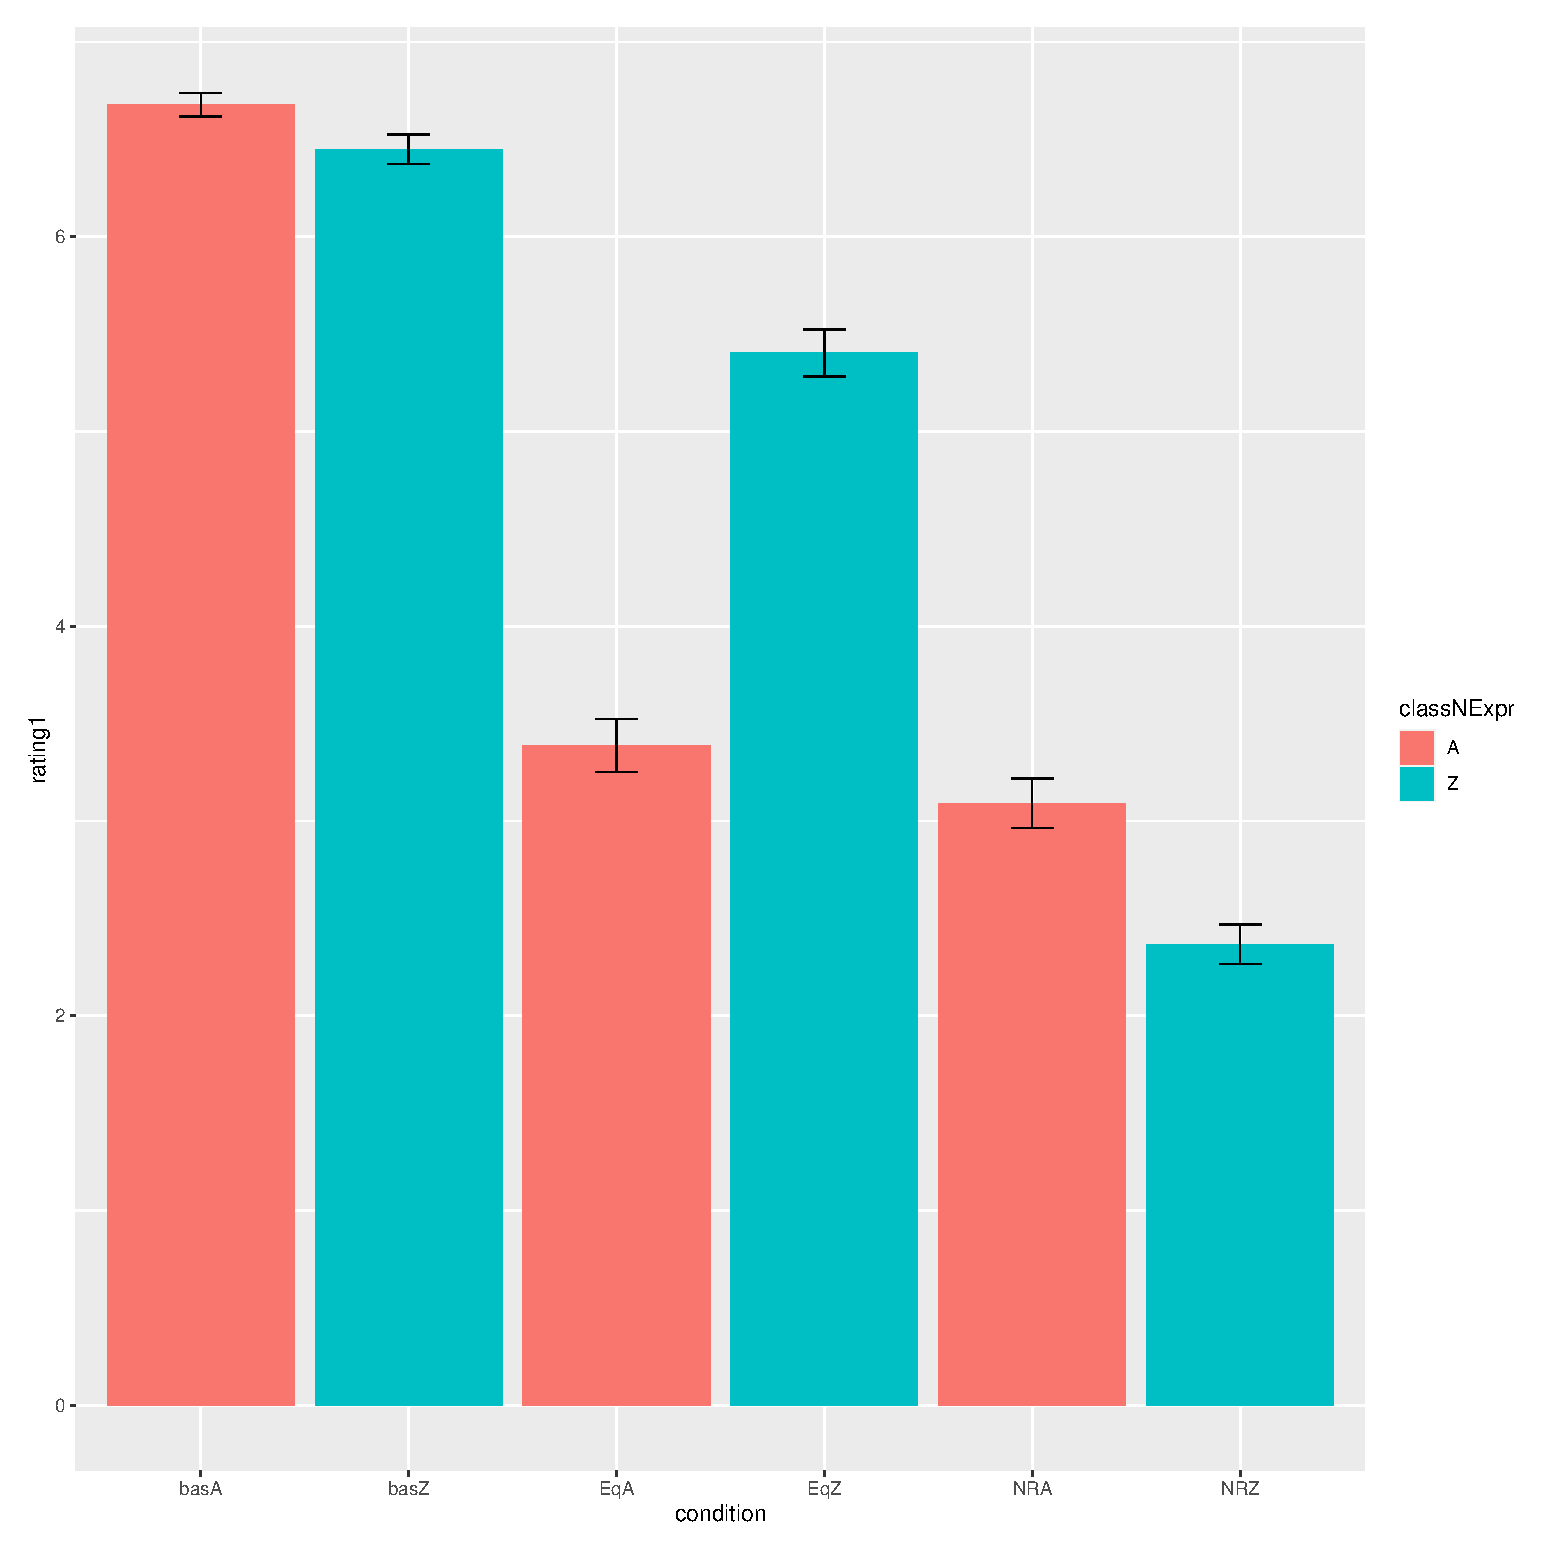
\includegraphics[scale=0.4]{error_bar_without_prob.eps}
  \label{fig-error-bar}
\end{figure}

The Bayesian hierarchical random-effects model with default priors was fit using the R package \textsc{rstanarm} \citep{rstanarm}: the dependent variable was the subject's response; the independent variables were: (i) environment (\textsc{bas, eq, nr}), (ii) type of the polarity-dependent expression (\textsc{a, z}), and their interaction; the reference level was \textsc{bas, a}. The model included random effects for both subject and item intercepts.

Using the model, we found that (i) baseline was very well accepted ($\mathrm{Intercept}=6.67$, 95 \% C(redibility) I(nterval)$=[6.38, 6.95]$), there is no distinction between neg-words and strong NPIs in it and sine qua non, both expressions are acceptable to the same extent (posterior main effect in the form of median and 95 \% CI: $\hat{\mu}=-0.20$, $\mathrm{CI}=[-0.47, 0.08]$), (ii) neg-words were much better accepted in equatives than strong NPIs (the positive interaction of \textsc{eq} by \textsc{z}: $\hat{\mu}=2.18$, $\mathrm{CI}=[1.81, 2.58]$), (iii) strong NPIs were preferred in Neg-Raising (the negative interaction of \textsc{nr} by \textsc{z}: $\hat{\mu}=-0.53$, $\mathrm{CI}=[-0.91, -0.14]$). The results are also supported by the results of R(egion) O(f) P(ractical) E(quivalence), ROPE: only \textsc{z} is not significant, since it is 23 \% in ROPE. For all medians, confidence intervals, and ROPE percents, see \tabref{tab:exp1}, all percents of ROPE are computed for the interval $[-0.10, 0.10]$. Medians, 95\% credibility intervals, and ROPE are also visually represented by the graph in \figref{fig-rope}.



\begin{table}[htbp]
  \centering
  \begin{tabularx}{.9\textwidth}{lrrrr}
  \toprule
  \textbf{Parameter}&\\\midrule
    &            Median & CI &  \% in ROPE\\  
    Intercept               &$6.67$   &$[6.38,6.95]$ &$0\%$\\  
    \textsc{Eq}               &$-3.27$   &$[-3.53,-3.00]$ &$0\%$\\  
    \textsc{nr}               &$-3.57$   &$[-3.86, -3.30]$ &  $0\%$\\  
    \textsc{z}               &$-0.20$   &$[-0.47,  0.08]$ &$23.08\%$\\  
    \textsc{Eq:z}               &$2.18$   &$[1.81,  2.58]$   &$0\%$\\
    \textsc{nr:z}               &$-0.53$   &$[-0.91, -0.14]$   &$0\%$\\  
    \bottomrule
    \textbf{Random effects}&\\\midrule
    & Name &SD\\
    subject&Intercept&$0.57$\\
    item&Intercept&$0.35$\\
  \bottomrule
  \end{tabularx}
  \caption{Bayesian model and its posterior distribution for the experiment}%; log-likelihood: -638.5
  \label{tab:exp1}
\end{table}

\begin{figure}
  \centering
  \caption{Graph of posterior samples with ROPE (for the experiment)}
  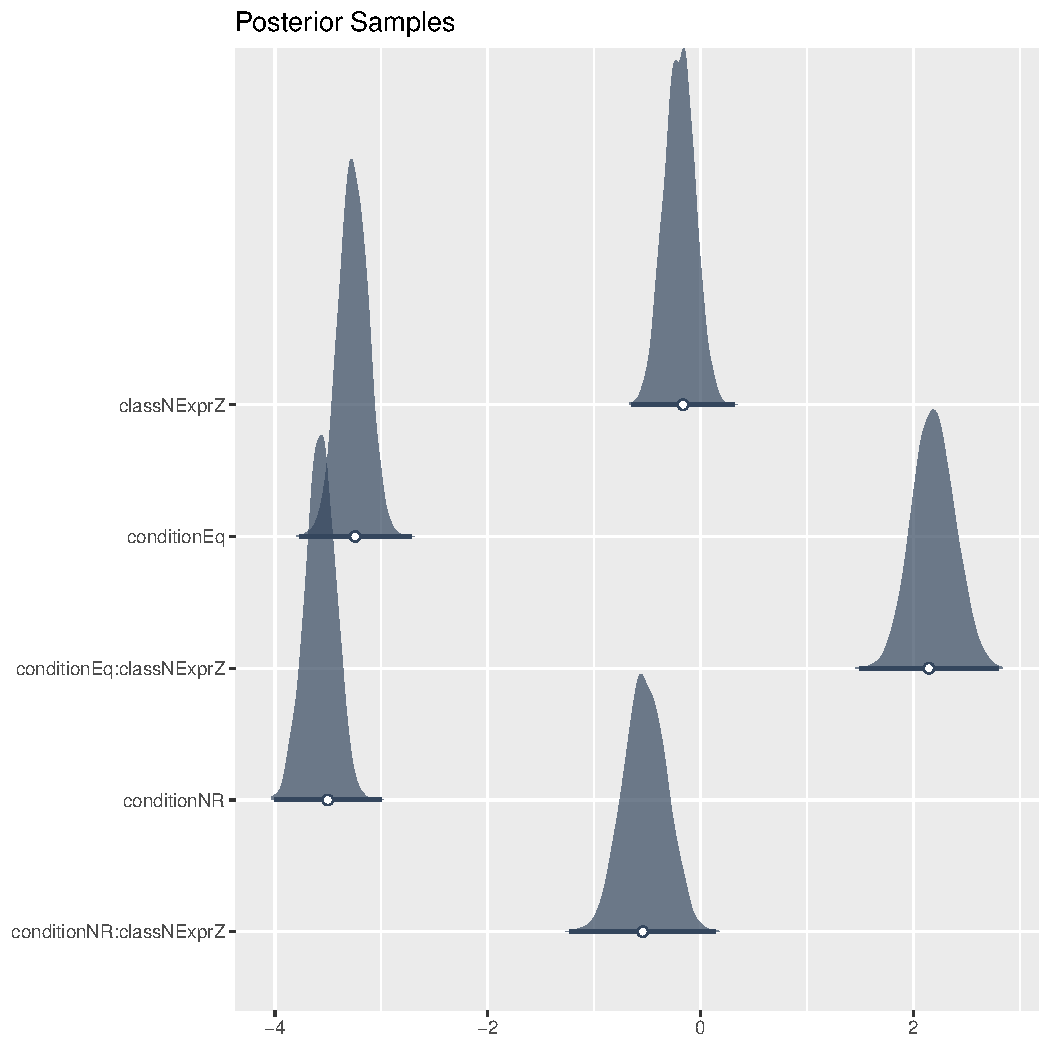
\includegraphics[scale=0.6]{posterior_graph.pdf}
  \label{fig-rope}
\end{figure}

\subsection{Demographic factors}

Next, three Bayesian generalized mixed linear models were fitted to detect any demographic factors inhibiting or prohibiting the acceptability. This was important since previous work (see \citealt{burnett2015variable} and \citealt{burnett2018structural} a.o.) revealed that both grammatical and demographic factors are at play when negative polarity variation is linguistically studied. As a reminder: the experiment included three demographic questions: region, age, and daily reading time. The last factor was used as a proxy for investigating the educational level. But it has to be said that the pool of subjects was rather homogeneous, consisting mainly of university students. Therefore, the education level results should be taken with a grain of salt and mainly as a first step in the general description of polarity items variation in Slavic languages.

Let's start with \textsc{age}. Descriptively, \textsc{age} ranged from 19 to 71, with a median 23, mean 25.59, and sd 9.47. The age was first z-transformed and then plugged in as the third interaction variable in the Bayesian model (next to the two conditions, \textsc{z} and \textsc{bas/nr/eq} environment). The model revealed that the acceptability overall wasn't affected by age at all (main effect of \textsc{age}: $\hat{\mu}=0.01$, $\mathrm{CI}=[-0.25,  0.28]$, ROPE: $58.00\%$ for the $[-0.10, 0.10]$ interval). There was also no significant interaction with any single or pair of conditions. The lowest ROPE was 30.55 \% for the three-way interaction between \textsc{Eq:Z:age}. All other interactions had an even bigger portion in ROPE and were also less significant.

Next, \textsc{region} was more varied than \textsc{age} where the data points from the first to the third quantile were in the range 21 to 25. But since I didn't control for the specificity of the values entered into the form, the answers ranged from city-specific to region-specific. For this reason, I aggregated all the answers into discrete factor with two levels: \textsc{Moravian, nonMoravian}. 67 \% of subjects entered as their region \textsc{nonMoravian}, the remaining 33 \% identified themselves as being from Moravia. Again the factor \textsc{region} was used as the third interaction variable in the Bayesian model. The main effect of the region wasn't significant ($\hat{\mu}=0.33$, $\mathrm{CI}=[-0.18,  0.88]$, ROPE: $14.79\%$ for the $[-0.10, 0.10]$ interval) but this time there was some anecdotal evidence coming from interactions. Namely, there seems to be a slight tendency for higher acceptance of Neg-Raising in the non-Moravian part of the Czech Republic (the interaction \textsc{nr:Moravian}: $\hat{\mu}=-0.61$, $\mathrm{CI}=[-1.28,  0.04]$, ROPE: $3.89\%$ for the $[-0.10, 0.10]$ interval). All other interactions with \textsc{region} were less significant. Still, even the \textsc{nr:region} is so weak that I doubt there is any genuine linguistic Neg-Raising isogloss between Czech dialects.

The last demographic factor was reading time. As hinted above, the factor was used to get information about education or education aspirations. The answers (converted to hours) ranged from 0 to 10 hours, with 1 hour as the median, 1.43 hours as the mean, and the range of first and third quantiles being 1 hour and 2 hours, respectively. Similarly to \textsc{age}, data points are centered around the mean with a small standard deviation, 1.26, and few outliers. As in the case of \textsc{age}, I recoded the continuous variable as a factor \textsc{readingTime} with two levels: \textsc{over1hour,under1hour} dividing the sample according to the median value of reading time. The result was two nearly proportional halves: 52 \% of subjects claimed that their daily reading time is under 60 minutes, and the remaining 48 \% entered that they read more than one hour. And again, as with two previous demographic factors, the main effect of \textsc{readingTime} is nonsignificant ($\hat{\mu}=-0.13$, $\mathrm{CI}=[-0.63,  0.39]$, ROPE: $28.89\%$ for the $[-0.10, 0.10]$ interval). And similarly to \textsc{age}, there was one weakly significant interaction: subjects claiming to read more than average (over 60 minutes daily) are more accepting Neg-Raising constructions (\textsc{nr:over1hour} interaction: $\hat{\mu}=0.66$, $\mathrm{CI}=[ 0.04,  1.27]$, ROPE: $1.24\%$ for the $[-0.10, 0.10]$ interval). All other interactions were much less significant.

Let's summarize: the design of the experiment and three demographic questions didn't reveal any important information concerning the demography-related variation in polarity constructions of Czech speakers. Two weak effects can be interpreted as clues about region and education-level variation concerning Neg-Raising. Still, there seems to be nothing significant in the variation of \textit{ani} vs. \textit{žádný} in the studied constructions. So, whatever speaker variation (in the usage of \textit{ani}) we will discuss further, it seems not to be derivable from age, region, or education level (unlike in the previous work like \citealt{burnett2015variable,burnett2018structural}).


\subsection{Correlations}

The Bayesian model revealed that both non-baseline environments (\textsc{nr} and \textsc{Eq}) were less accepted by speakers, but there was no difference between \textit{ani} and \textit{žádný} in terms of main effects. Nevertheless, speakers accepted in equatives much more neg-words than strong NPIs (the strong and only one positive interaction effect). But speakers are also inclined to reject neg-words in Neg-Raising against strong NPIs (the negative interaction effect between \textsc{z} and \textsc{nr}). The theoretical consequences of these findings will be discussed below, but let's turn to another kind of variation, this time not demographic.

The first important thing to note is that all speakers agreed on their high acceptance of baseline and in this condition they accepted neg-words and strong NPIs indistinguishably. But this acceptance of both polarity expressions diverged in the two other conditions. Namely, some speakers rate \textit{ani} high in equatives (unlike the main thrust of speakers, recall that the strong positive interaction between \textsc{z} and \textsc{Eq}) but also reject it in NegRaising (again going against the overall acceptance of strong NPIs there: the negative interaction between \textsc{z} and \textsc{nr}). And vice versa: subjects who reject strong NPIs in equatives (behaving according to the negative interaction effect) accept strong NPIs in Neg-Raising (again verifying the negative interaction effect). In both cases, we observe a negative correlation between the acceptability of neg-words/strong NPIs in the two environments, equatives, and Neg-Raising. One way to understand this reversed correlation is to assume that for the first kind of speakers (those who accept \textit{ani} in equatives) is \textit{ani} more like neg-word and not strong NPI. The rest of the sample (majority, in fact) treats \textit{ani} as strong NPI and therefore accepts it under Neg-Raisers and rejects it in equatives.

The way the correlations were checked statistically is the following. First, the acceptance of conditions was z-transformed (by subject). And then, such z-transformed variables were checked for correlations across conditions. And indeed, there is a strong negative correlation between the acceptability of \textit{ani} in equatives and its acceptability under Neg-Raising predicates (Pearson's product-moment correlation: $t = -5.93, p < 0.001$). The correlation graph is in \figref{fig-ani-corr}. This means that we can identify two groups of speakers: (i) speakers who accept \textit{ani} under Neg-Raisers and reject it with equatives (top left section in the \figref{fig-ani-corr}), (ii) speakers who accept \textit{ani} in equatives and reject it under Neg-Raisers (the bottom right part of \figref{fig-ani-corr}). But crucially, no speakers are accepting both conditions (the empty top right corner) nor speakers who would reject both conditions (the empty space in the bottom left part). And also, there is no correlation between the acceptability of \textit{ani} acceptability in the baseline and equatives, just pure noise as can be seen in \figref{fig-ani-bas-corr}. This correlation of \textit{ani} between \textsc{nr} and \textsc{Eq} resonates the previous work \cite{docekaldotlacilsubber} where similar correlations were found (for \textit{ani}) in the case of probability manipulated conditions and Neg-Raising.

Let's summarize: the experiment results show that Czech strong NPIs are (for most speakers) accepted under Neg-Raising predicates and rejected in equatives. For Czech neg-words, the opposite is true: most speakers accept them in equatives but reject them under Neg-Raising predicates. In the case of \textit{ani} (strong NPI), there is a speaker variation, and some subset of speakers treats it more like a neg-word; nothing similar was found for neg-words. Moreover, the speaker variation doesn't seem to be derivable from demographic factors (or at least not from the demographic factors controlled in the experiment).

\begin{figure}
    \centering
    \caption{Correlations between Equatives and Neg-Raising for \textit{ani}}
    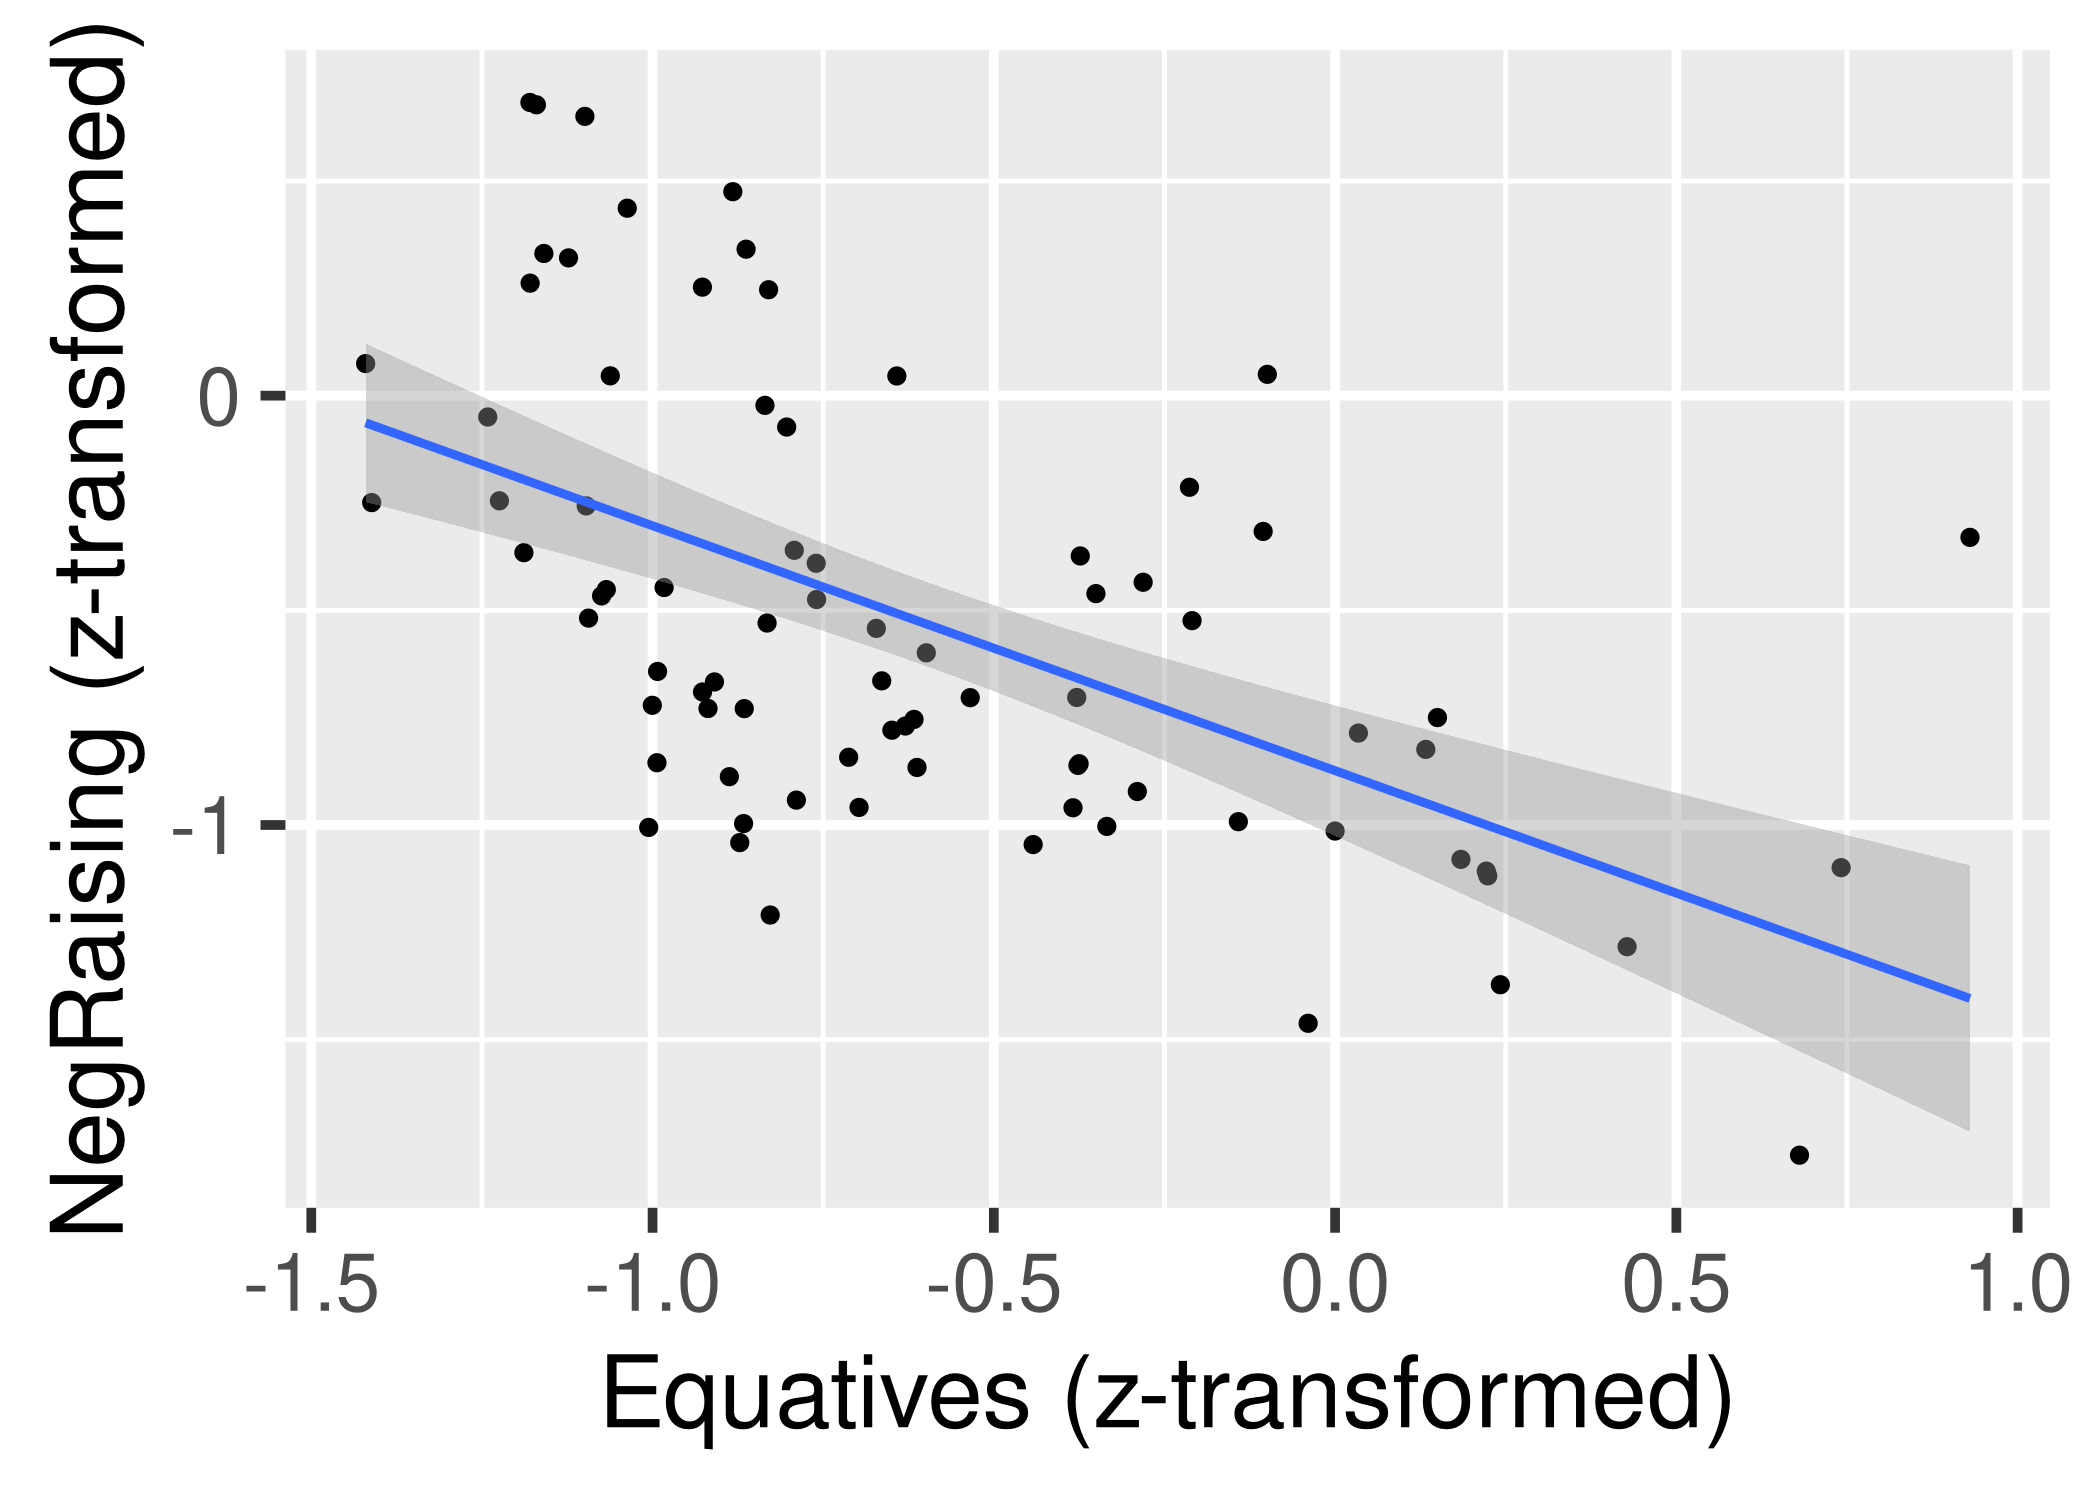
\includegraphics[scale=0.6]{correlations_ani.png}
    \label{fig-ani-corr}
\end{figure}
  
\begin{figure}
  \centering
  \caption{Correlations between Equatives and Baseline for \textit{ani}}
  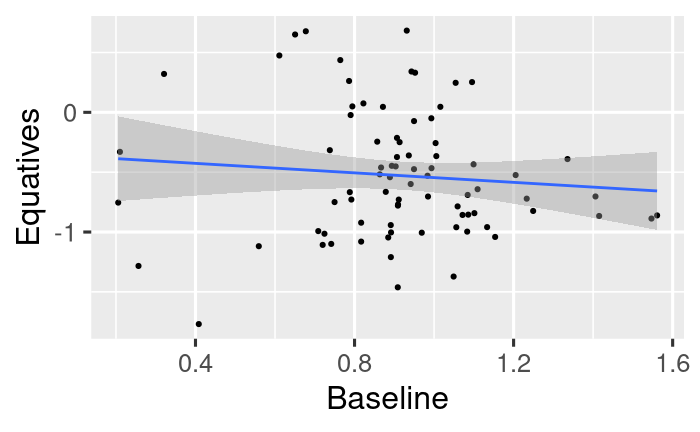
\includegraphics[scale=0.6]{equatives_baseline_corr.png}
  \label{fig-ani-bas-corr}
\end{figure}

\section{Theoretical consequences}\label{sec:theoretical_consequences}

The nature of this article is mainly experimental. For this reason and the obvious constraints of space, the consequences of the analyzed experimental data will be discussed only to a limited extent. 

\subsection{Assumptions: licensing of (strong)
NPIs}\label{sec:assumptions-licensing-of-strong-npis}

Let's assume a standard approach to NPIs and strong NPIs licensing. For the general framework, the so-called \textit{even}-theory of NPIs licensing is naturally the most attractive candidate, see \citet{krifka1995semantics,lahiri1998focus,crnivc2014non} a.o., since \textit{ani} bears the unlikelihood presupposition similar to English \textit{even}. And for strong NPIs, let's follow Gajewski's formalization of strong NPIs,  \citet{gajewski2011licensing}. According to \citet{gajewski2011licensing}, strong NPIs are licensed in downward-entailing (DE) environments. But the downward-entailments are checked both in Truth-Conditions (TC), the at-issue part of the meaning, and in the non-at-issue meaning, presuppositions and implicatures being the most pertinent non-at-issue meaning components. Weak NPIs, on the other hand, require DE environments only in the TC part of the meaning. The conditions for weak and strong NPIs are summarized in \REF{ex:9}.

\ea\label{ex:9} An NPI is licensed in the environment \(\gamma\)\\
\([_\alpha exh [_\beta \ldots [_\gamma\) NPI \(] \ldots ]]\): 
\ea the environment \(\gamma\) is DE in \(\beta\) \hfill weak NPIs 
\ex the environment \(\gamma\) is DE in \(\alpha\) \hfill strong NPIs\z\z

The standard exhaustifier from \REF{ex:9} is the formalization of \textit{only}-kind of focus operator which works very well for weak NPIs like unstressed English \textit{any}. But for other weak or strong NPIs with the unlikelihood presupposition meaning core, another kind of exhaustifier, a namely covert counterpart of English \textit{even} was proposed (see \citealt{crnic2011getting,crnivc2014against}). The same mechanism is used in formal approaches to focus particles; see \citet{panizza2020minimal}. The \textit{even} exhaustifier, like its overt version, then comes with two presuppositions: first is scalar, demonstrated in \REF{ex-10-a} -- the sentence is acceptable in such contexts where dancing Pope is very unlikely (compatible with the actual world). The second is additive, exemplified with \REF{ex-10-b}. The sentence is true if two, three, \ldots cats will make Pope happy as well. The placement of focus determines the nature of alternatives used in presuppositions. Let's follow the formalization of both presuppositions by \citet{panizza2020minimal}, see \REF{ex-11}. For monotonic scales, likelihood from \REF{ex-11} translates into entailment (after \citealt{crnic2011getting}), therefore the predictions of traditional downward entailing approaches like \citep{ladusaw1992expressing} and \textit{even}-theories of NPIs collapse for downward monotonic contexts.


\ea\label{ex-10} \ea\label{ex-10-a} Even Pope\(_F\) danced. 
\ex\label{ex-10-b} Even one\(_F\) cat will make Pope happy.\z\z

\ea\label{ex-11} `Even \(\phi\)' presupposes: 
\ea that \(\phi\) is relatively unlikely to be true among Alt(\(\phi\)); and 
\ex that there is \(\psi \in\) Alt(\(\phi\)) that is not entailed by \(\phi\) and is true.\z\z

Now, let's demonstrate how the \textit{even}-approach applies to Czech data from the experiment, starting with the baseline. As discussed above, \textit{ani} comes with the \textit{even}-presuppositions, namely the scalar and the additive. In the formal terms, this is cached as an association of \textit{ani} with covert \textit{even} scoping at the propositional level; see a schematic representation of the baseline in \REF{ex-12} and its logical form in \REF{ex-12-a}. Since the sentence is negated, the entailment between numerals is reversed by negation:
\(\neg (\llbracket\) one cat \(\rrbracket \ldots) \models \neg(\llbracket\)two
cats\(\rrbracket \ldots)\). The sortal type of the alternatives, other cardinality predicates in this case, comes from the focus since \textit{ani} can associate with nouns, clauses, etc. Because the entailment is reversed, the \emph{even}-approach predictions agree with the downward-entailing explanation. Moreover, since \textit{ani} is a strong NPI, it requires DE/\textit{even}-presuppositions to be satisfied both in truth conditions (configurationally $\beta$ in \REF{ex-12-a}) but also at the level of non-at-issue meaning (where the exhaustifier scopes: $\alpha$ in \REF{ex-12-a}). Next, we have to check both presuppositions as schematically formalized in \REF{ex-12-d} and \REF{ex-12-e}, which is also fulfilled.

  
\ea\label{ex-12} Ani one thief neg-remained in the kingdom.\\
\ea\label{ex-12-a} ~{[}\(_\alpha\) (\(even\)) {[}\(_\beta\)
  \neg [$_\gamma$ ani one thief remained in the kingdom ]{]} {]} 
\ex TC  (in \(\beta\)) DE: \(\checkmark\) 
\ex non-at-issue (in \(\alpha\)) DE:
  \(\checkmark\) 
\ex\label{ex-12-d} scalar presupposition of (even): \(\rightarrow\)
  \(\neg\)(two thieves remained), \(\neg\)(three thieves remained),
  \ldots: \(\checkmark\)
\ex\label{ex-12-e} additive presupposition: \(\neg\)(two thieves
  remained) \(\vee\) \(\neg\)(three thieves remained), \ldots:
  \(\checkmark\) \z\z

Continuing now to the Neg-Raising condition. Neg-words were in \textsc{nr} less accepted than strong NPIs; although the effect wasn't particularly strong, it was still significant. To explain the \textsc{nr} results, we can adapt any current theory of Neg-Raising, be it the presuppositional version of \citet{gajewski2007neg} or the scalar implicature version of \citet{romoli2013scalar}. Both share the insight that Neg-Raising predicates bear the excluded middle inference: for \textit{believe}: $Bel(p) \vee Bel(\neg p)$, adding the negated assertion $\neg Bel(p)$ results in the deductively valid conclusion where the negation scopes in the embedded clause, $Bel(\neg p)$. Non-Neg-Raising predicates then come without the excluded middle inference resulting in the surface interpretation of the negation. But for Neg-Raising predicates like \textit{chtít} `want' from the experiment, then the schematic scope configuration in the embedded clause is covert (\(even\)) \textgreater{} \(\neg\) \textgreater{} {[}\ldots{} one \ldots{]} and the explanation from the baseline condition applies here. The preference for strong NPIs vs. neg-words seems to come from locality constraints since neg-words' licensing has a strong syntactic component.

\subsection{Neg-words}

This section introduces the core ingredients of the semantic/pragmatic theory of neg-words and negative concord. It is an alternative to the standard, syntactic theory introduced above. It was formulated in \citet{ovalle2004double}, and a modern reformulation can be found in \citet{kuhn2022dynamics}. It shares some assumptions with the syntactic theory though. First, both theories agree on the indefinite description status of neg-words. Therefore neg-words denote sortally existential quantifiers like in \REF{ex-13-a}. The negative force, which in the syntactic theory is carried by the covert Op, is in the semantic/pragmatic theory reformulated as a presupposition of empty reference in the original version, \REF{ex-13-b}. Or in the dynamic reformulation as a test on the cardinality of discourse referents like in \REF{ex-13-c}. In this article, we can abstract away from the formal implementations and work with the core assumption: the emptiness of reference is a presupposition with the usual projection properties of presuppositions. 

\ea\label{ex-13} \ea\label{ex-13-a} \(\llbracket\)neg-word\(\rrbracket\)=\(\lambda P.\exists x[SORT(x) \wedge P(x)]\)
  \hfill TC 
\ex\label{ex-13-b}   \(\llbracket\)neg-word\(\rrbracket\)=\(\neg \exists x[SORT(x) \wedge P(x)]\)
  \hfill non-at-issue 
\ex\label{ex-13-c} after \textcite{kuhn2022dynamics}:
  \(\wedge \mathbf{0_x}\) \ldots postsupposition (highest scope) \z\z
  
The original version of the semantic/pragmatic theory doesn't come with any locality constraints on the neg-words licensing, which is a problematic assumption since negative concord is in most cases limited to the clause-internal dependency between neg-words and verbal negation, e.g., This also one of the reasons why the syntactic approach is so successful and remains the standard theory of neg-words today. \citet{kuhn2022dynamics} improves in many aspects over the original version of the semantic/pragmatic theory, one of them is the delimitation of the emptiness of reference presupposition in terms of previous contexts and also in tying it to discourse referents and therefore making the presupposition more specific. But most importantly, \citet{kuhn2022dynamics} brings some syntactic constraints into the game. He formalizes neg-words' syntax via split-scope around their licensor (prototypically negation). Since the split scope is realized via quantifier raising, some locality constraints on the neg-word emerge. More specifically, \citepossalt{kuhn2022dynamics} empirical claim is that the locality constraints on neg-words licensing should correspond to the locality of quantifier raising in the particular language and construction. Whether this is, the right theoretical solution is a separate question, which is not answerable in this article. Still, it is definitely a step in the right direction: including some form of syntactical sensitivity for locality into the semantic/pragmatic theory.

The baseline can now be explained easily. In a negative sentence, like schematic \REF{ex-14}, the truth conditions (indefinite descriptions) of the neg-word and its presupposition agree: the indefinite description is under the scope of negation, and the presupposition of the emptiness of the discourse referent are in accord. But in a positive sentence like \REF{ex-15}, the existential quantification over the discourse referent and the presupposition of its reference emptiness would clash. 


\ea\label{ex-14} neg-word thief neg-remained in the kingdom. \ea {[}\(\neg[\exists x[\mathsf{thief}(x) \wedge \mathsf{remained}(x)]\) {]}{]} \(\wedge \mathbf{0_x}\)\z\z

\ea\label{ex-15} neg-word thief remained in the kingdom. \ea {[}\(\exists x[\mathsf{thief}(x) \wedge \mathsf{remained}(x)]\) {]} \(\wedge \mathbf{0_x}\) \hfill \(\bot\)\z\z

Turning now to Neg-Raising: neg-words were less accepted in \textsc{nr} than strong NPIs. From the perspective of the semantic/pragmatic theory of neg-words, we should expect that this would align with the quantifier raising. Reformulated empirically: Czech speakers should be reluctant in interpreting Czech translation of \REF{ex-16} with the wide scope of $\forall$ over the indefinite description \textit{one teacher} to the same extent as they would be reluctant to license neg-words under negated Neg-Raising \textit{chtít} `want.' Whether this is, an empirically correct claim is a question for future work. But let's assume that such a correlation is possible. Then we have a handle on neg-word unacceptability under Neg-Raising predicates: the locality constraint (similar to quantifier raising limitation) prohibits the split-scope transformation of the neg-word over the root negated predicate and leaving it in its base position, leads to the same kind of problems like \REF{ex-15} faces.

\ea\label{ex-16} One teacher doesn't want every student to pass the exam.
\z

Finally, I will comment on the relationship between current theories of equatives and their predictions concerning strong NPIs. The first thing to note is that the standard theory of equatives is built on the the `>' analysis of comparatives \citep{beck_comparison_nodate,stechow1984comparing} where the core operation is the relation > comparing two maxima: (i) the maximum of the set of degrees from the main clause, (ii) the maximum of the set of degrees from the complement of the comparative clause, see \REF{ex-17} as an illustration. 


\ea\label{ex-17} The dog is taller than the cat. \ea MAX({$d$\vert the height of the dog $\geq d$}) > MAX({$d$\vert the height of the cat $\geq d$})\z\z

The standard theory of equatives \citet{beck_comparison_nodate,stechow1984comparing,rullmann1995maximality} then follows the `>' analysis of comparatives, just replacing > with $\geq$ which is in most context pragmatically strengthened to `=', see \REF{ex-18} for an illustration. The comparatives are then theoretically expected to license NPIs in their complement clauses since the degree argument is downward-monotonic, therefore if some degree $d > d'$ and there is another degree $d''$, such as $d' > d''$, then by transitivity $d > d''$. Intuitively: if the dog from \REF{ex-17} is taller than the cat from \REF{ex-18}, then he is taller than any cat smaller than the cat. This is routinely checked in the comparative literature by \citep{stechow1984comparing,rullmann1995maximality,gajewski2008more} the licensing of weak NPIs (like English \textit{any}) in the complement clauses of the comparative which seems to work well. In the case of strong NPIs, the empirical situation is less clear. Still, at least empirically, it is claimed for Germanic languages that strong NPIs appear in the complement clause of comparatives felicitously; see Dutch \citepossalt{hoeksema2008natural} example in \REF{ex-19}. \REF{ex-19} contains the Dutch expression \textit{ook maar} `even,' which is taken as a standard example of a strong NPI, see \citet{zwarts1998three}.

\ea\label{ex-18} The dog is as tall as the cat. \ea MAX({$d$\vert the height of the dog $\geq d$}) $\geq$ MAX({$d$\vert the height of the cat $\geq d$})\z\z

\ea\label{ex-19} \gll Zij was beter dan ook maar iemand verwacht had.\\
she AUX better than strong NPI {} expected AUX\\
\glt `She was better than anyone could have expected.'
\z

As for equatives, they are theoretically expected to license NPIs which seems to be the case for English weak NPIs as illustrated by \REF{ex-5}. But it was noticed before that this doesn't hold cross-linguistically, see \citet{krifka1992some} for German and \citet{penka2016degree} for German and Romance languages. But at least in the comparative/equative `>' theories, if comparatives license strong NPIs, the expectation is that equatives will behave similarly. Turning now to Slavic equatives, there are many factors at play here, though. First, Slavic equatives are different from English equatives, and their morpho-syntax is very similar to correlatives (as German and Romance equatives). And since it is known at least from \citet {pauline1995quantificational} that correlatives are bad licensors of NPIs, the expectation is that both weak and strong NPIs will be much worse in Slavic equatives (compared to Germanic languages). To address this issue, another experiment targeting both weak and strong NPIs in comparatives and equatives is in preparation. But to wrap up: (i) as tested in the experiment, neg-words are, but strong NPIs are not acceptable in the complement clause of the Czech equatives, (ii) adding to this, verbal negation is not acceptable either -- see \REF{ex-20}. Especially the high acceptability of neg-words is surprising from the Germanic perspective since negative quantifiers are distinctly odd in this position, see \REF{ex-21} from \citet{gajewski2008more}.

  
\ea\label{ex-20} \gll Petr je tak chytrý jak \minsp{\{} nikdo jiný / *Marie ne / *ani jeden\}.\\
Petr is so smart as {} neg-word else {} Mary not {} strong NPI\\
\glt `Petr is as smart as anyone.'
\z  

\ea\label{ex-21} *Mary is taller than no boys are.
\z
  
The ambition of this article is not to solve the above-mentioned theoretical puzzles. But let's at least indicate how a possible solution can be. The experiment results show that neg-words are very much accepted in the complement clause of equatives, while strong NPIs are degraded there. Moreover, intuitions and preliminary results from the follow-up experiment suggest that weak NPIs are not acceptable in the equatives either, following the German and Romance data discussed in \citet{krifka1992some,penka2016degree}. The emerging picture seems that Czech complement clauses of equatives are not downward-monotonic in either truth conditions or non-at-issue meaning. But for some reason, the emptiness of the neg-words' discourse referents presupposition can be easily satisfied in this environment. This can be compatible with \citepossalt{penka2016degree} suggestion to replace the MAX operator in analyzing English equatives with a different relation on the degrees. But so far, I consider the evidence to be non-conclusive regarding the monotonic properties of Czech complement clauses of equatives; they're not downward entailing for sure, but the resulting two possibilities: upward entailing or non-monotonic, are still open. Theoretically wise, I agree with \citet{penka2016degree} that current degree theories of equatives don't hold the cross-linguistic water. And in the same direction, it's clear that a purely syntactic approach to neg-words faces big trouble when posed with the acceptability of neg-words in equatives. Whatever theoretical change in the theory of equatives is possible (using MAX$_{inf}$ as suggested by \cite{penka2016degree}, e.g.), there is clearly no room for sentential negation operator in its formula since then the weak or strong NPIs would be admissible there, contrary to facts.


% First, I will foll \citet{penka2016degree} in taking the morphosyntactic clues seriously and replace the standard `>' theory MAX operator with \(max \rightarrow max_{inf}\), corresponding to the operator used in the analysis of correlatives. The logical form for a schematic \textsc{eq} like \REF{ex-22} is in \REF{ex-22-a}. Czech \textit{tak} `so' is anaphoric to the degree from the main clause, \REF{ex-22-b}. Then the neg-word presupposition (from the semantic/pragmatic theory of neg-words) has to be satisfied: \REF{ex-22-d}.

%   \begin{itemize}
  
%   \item
%     syntactic and semantic ingredients (pseudoCzech in NEXT)
%   \item
%     non-standard: \(max \rightarrow max_{inf}\) (otherwise \(max\) would
%     lead to \(\bot\)): \cite{penka2016degree}
%   \end{itemize}

%   Motivation of the ingredients:
  
%   \begin{itemize}
  
%   \item
%     \(max_{inf}\): the equative in Czech has exactly the same building
%     blocks (\emph{tak} `so' \ldots{} \emph{jak} `how') as correlative
%     constructions
%   \item
%     \emph{other}: the anaphor similar to reciprocal anaphors
  
%     \begin{itemize}
    
%     \item
%       it identifies the dref
%     \item
%       it is also used in the exceptive phrases from which the
%       presupposition comes: \emph{Nobody other than John neg-came}
%       presupposes that John came (as the only exception)
%     \end{itemize}
%   \item
%     neg-word presupposition ranges over the dref picked up by the
%     reciprocal
%   \end{itemize}
  
 

% LOOK AT IT AGAIN

% \ea\label{ex-22} This thief is so clever how neg-word other thief.\\
%   \ea\label{ex-22-a} {[} so {[}so\(_1\) no other thief \(t_1\) clever {]}{]}\(_2\)
%   {[}This thief is \(t_2\) clever{]}\\
%   \ex\label{ex-22-b} \(\llbracket so\rrbracket\) \ldots{} picks up the degree denoted by
%   the standard clause\\
%   \ex\label{ex-22-c} \(\llbracket\) so\(_1\) neg-word other thief clever is
%   \(\rrbracket\)\\
%   \ex\label{ex-22-d} nobody other than the thief is \(d\)-clever \hfill neg-word
%   presupposition\\
%   \ex the thief is \(d\)-clever \hfill implicature of \emph{other}\\
%   \z\z
  
%   \ea \ea \(\llbracket\) as
%   \(\rrbracket = \lambda S\lambda C.max(C) \geq max(S)\)\\
%   \ex
%   \(S' \subseteq S: max(C) \geq max(S) \rightarrow max(C) \geq max(S')\)
%   \hfill English DE \textit{as}\z\z
  
\section{Summary}\label{sec:summary}  

This section summarizes the experiment's results and adds some related theoretical consequences. First, we can answer research question 1, repeated below as \REF{ex-22}. For neg-words, it seems nearly sure that their acceptability in the complement clauses of equatives is derived from their presupposition relativized to the set of degrees introduced in the main clause. Neg-words in examples like \REF{ex-20} are well accepted since, in this configuration; the presupposition doesn't require total emptiness of reference, just the emptiness of reference for such discourse referents whose degree would exceed the degree of the subject. Next, the strong NPI unacceptability is a direct consequence of the Czech equatives complement clauses not being downward monotonic. The sub-answers to research question 1 are in \REF{ex-23}.

\ea\label{ex-22} How to explain the unpredicted acceptability of neg-words in the complement clauses of Czech equatives (and strong NPIs unavailability there)?
\z

\ea\label{ex-23} The non-standard theories of negative concord and equatives give promising answers:\\
  \ea The semantic/pragmatic theory of neg-words allows the presupposition of discourse emptiness to be satisfied (relativized to degrees of the main clause).\\
  \ex The complement clause of the Czech equatives isn't downward entailing.\z\z

Now, research question 2 is repeated below as \REF{ex-24}. Despite observing the speaker variation: recall, that for some speakers \textit{ani} behaved more like neg-word, it is unlikely that the variation can be related to demographic factors such as age, region, or daily reading time. But there's one way to theoretically explain the variation: we can assume that both neg-words and strong NPIs in Czech come with presuppositions, the emptiness of discourse referents for neg-words, and scalar for strong NPIs. Then the flux from strong NPIs to neg-words can be theoretically cashed out by substituting the scalar presupposition with the scalar presupposition. Speculatively, we can try to explain the one-way direction in terms of economy: the scalar presupposition needs a covert exhaustifier, but the emptiness presupposition doesn't. Therefore it is less costly and more attractive for speakers who oscillate between the two presuppositions. Why the flux isn't related to the demographic factors is an issue for future work. The answers are summarized in \REF{ex-25}.

  
\ea\label{ex-24} Question2: \ea How can we explain microvariation by grammatical
  (semantic) factors? \ex Is part of the variation caused by social
  factors? \z\z
  
\ea\label{ex-25} The speaker variation is explainable as shifting from the scalar to
  the emptiness of the DR presupposition (in case of \emph{ani jeden}
  `even one'). \ea Social factors don't seem to play a role in this shift.\z\z
  
Let's end this section with some open questions. The first of them concerns the locality constraints on neg-words licensing. The semantic/pragmatic theory predicts that the neg-word locality should approximate the quantifier raising. Only syntactic islands (such as relative clauses) should be hard limits for both neg-words licensing and quantifier raising. The syntactic literature on the topic of Slavic quantifier raising seems to argue for a possibility of overt movement (out of non-island clauses) but obligatory reconstruction (see \cite{neeleman2009focus} a.o.), but the experimental research in this direction seems to be limited to mono-clausal conditions (see \cite{ionin2018focus}, e.g.). So there is definitely space for future research in this direction, and only then can we conclude whether the locality constraints between quantifier raising and neg-words licensing really do coincide. Another open question concerns the cross-linguistic variation in neg-words licensing: in Romance languages, neg-words are licensed in \textit{before}-clauses and under \textit{doubt}-type predicates; in Slavic languages, this is not the case. The semantic/pragmatic theory of neg-words predicts that this should follow from the different presupposition projection properties in the two types of languages. Whether this is true remains again a question for future work.
  

% Just comment out the input below when you're ready to go.
% For a start: Do not forget to give your Overleaf project (this paper) a recognizable name. This one could be called, for instance, Simik et al: OSL template. You can change the name of the project by hovering over the gray title at the top of this page and clicking on the pencil icon.

\section{Introduction}\label{sim:sec:intro}

Language Science Press is a project run for linguists, but also by linguists. You are part of that and we rely on your collaboration to get at the desired result. Publishing with LangSci Press might mean a bit more work for the author (and for the volume editor), esp. for the less experienced ones, but it also gives you much more control of the process and it is rewarding to see the quality result.

Please follow the instructions below closely, it will save the volume editors, the series editors, and you alike a lot of time.

\sloppy This stylesheet is a further specification of three more general sources: (i) the Leipzig glossing rules \citep{leipzig-glossing-rules}, (ii) the generic style rules for linguistics (\url{https://www.eva.mpg.de/fileadmin/content_files/staff/haspelmt/pdf/GenericStyleRules.pdf}), and (iii) the Language Science Press guidelines \citep{Nordhoff.Muller2021}.\footnote{Notice the way in-text numbered lists should be written -- using small Roman numbers enclosed in brackets.} It is advisable to go through these before you start writing. Most of the general rules are not repeated here.\footnote{Do not worry about the colors of references and links. They are there to make the editorial process easier and will disappear prior to official publication.}

Please spend some time reading through these and the more general instructions. Your 30 minutes on this is likely to save you and us hours of additional work. Do not hesitate to contact the editors if you have any questions.

\section{Illustrating OSL commands and conventions}\label{sim:sec:osl-comm}

Below I illustrate the use of a number of commands defined in langsci-osl.tex (see the styles folder).

\subsection{Typesetting semantics}\label{sim:sec:sem}

See below for some examples of how to typeset semantic formulas. The examples also show the use of the sib-command (= ``semantic interpretation brackets''). Notice also the the use of the dummy curly brackets in \REF{sim:ex:quant}. They ensure that the spacing around the equation symbol is correct. 

\ea \ea \sib{dog}$^g=\textsc{dog}=\lambda x[\textsc{dog}(x)]$\label{sim:ex:dog}
\ex \sib{Some dog bit every boy}${}=\exists x[\textsc{dog}(x)\wedge\forall y[\textsc{boy}(y)\rightarrow \textsc{bit}(x,y)]]$\label{sim:ex:quant}
\z\z

\noindent Use noindent after example environments (but not after floats like tables or figures).

And here's a macro for semantic type brackets: The expression \textit{dog} is of type $\stb{e,t}$. Don't forget to place the whole type formula into a math-environment. An example of a more complex type, such as the one of \textit{every}: $\stb{s,\stb{\stb{e,t},\stb{e,t}}}$. You can of course also use the type in a subscript: dog$_{\stb{e,t}}$

We distinguish between metalinguistic constants that are translations of object language, which are typeset using small caps, see \REF{sim:ex:dog}, and logical constants. See the contrast in \REF{sim:ex:speaker}, where \textsc{speaker} (= serif) in \REF{sim:ex:speaker-a} is the denotation of the word \textit{speaker}, and \cnst{speaker} (= sans-serif) in \REF{sim:ex:speaker-b} is the function that maps the context $c$ to the speaker in that context.\footnote{Notice that both types of small caps are automatically turned into text-style, even if used in a math-environment. This enables you to use math throughout.}$^,$\footnote{Notice also that the notation entails the ``direct translation'' system from natural language to metalanguage, as entertained e.g. in \citet{Heim.Kratzer1998}. Feel free to devise your own notation when relying on the ``indirect translation'' system (see, e.g., \citealt{Coppock.Champollion2022}).}

\ea\label{sim:ex:speaker}
\ea \sib{The speaker is drunk}$^{g,c}=\textsc{drunk}\big(\iota x\,\textsc{speaker}(x)\big)$\label{sim:ex:speaker-a}
\ex \sib{I am drunk}$^{g,c}=\textsc{drunk}\big(\cnst{speaker}(c)\big)$\label{sim:ex:speaker-b}
\z\z

\noindent Notice that with more complex formulas, you can use bigger brackets indicating scope, cf. $($ vs. $\big($, as used in \REF{sim:ex:speaker}. Also notice the use of backslash plus comma, which produces additional space in math-environment.

\subsection{Examples and the minsp command}

Try to keep examples simple. But if you need to pack more information into an example or include more alternatives, you can resort to various brackets or slashes. For that, you will find the minsp-command useful. It works as follows:

\ea\label{sim:ex:german-verbs}\gll Hans \minsp{\{} schläft / schlief / \minsp{*} schlafen\}.\\
Hans {} sleeps {} slept {} {} sleep.\textsc{inf}\\
\glt `Hans \{sleeps / slept\}.'
\z

\noindent If you use the command, glosses will be aligned with the corresponding object language elements correctly. Notice also that brackets etc. do not receive their own gloss. Simply use closed curly brackets as the placeholder.

The minsp-command is not needed for grammaticality judgments used for the whole sentence. For that, use the native langsci-gb4e method instead, as illustrated below:

\ea[*]{\gll Das sein ungrammatisch.\\
that be.\textsc{inf} ungrammatical\\
\glt Intended: `This is ungrammatical.'\hfill (German)\label{sim:ex:ungram}}
\z

\noindent Also notice that translations should never be ungrammatical. If the original is ungrammatical, provide the intended interpretation in idiomatic English.

If you want to indicate the language and/or the source of the example, place this on the right margin of the translation line. Schematic information about relevant linguistic properties of the examples should be placed on the line of the example, as indicated below.

\ea\label{sim:ex:bailyn}\gll \minsp{[} Ėtu knigu] čitaet Ivan \minsp{(} často).\\
{} this book.{\ACC} read.{\PRS.3\SG} Ivan.{\NOM} {} often\\\hfill O-V-S-Adv
\glt `Ivan reads this book (often).'\hfill (Russian; \citealt[4]{Bailyn2004})
\z

\noindent Finally, notice that you can use the gloss macros for typing grammatical glosses, defined in langsci-lgr.sty. Place curly brackets around them.

\subsection{Citation commands and macros}

You can make your life easier if you use the following citation commands and macros (see code):

\begin{itemize}
    \item \citealt{Bailyn2004}: no brackets
    \item \citet{Bailyn2004}: year in brackets
    \item \citep{Bailyn2004}: everything in brackets
    \item \citepossalt{Bailyn2004}: possessive
    \item \citeposst{Bailyn2004}: possessive with year in brackets
\end{itemize}

\section{Trees}\label{s:tree}

Use the forest package for trees and place trees in a figure environment. \figref{sim:fig:CP} shows a simple example.\footnote{See \citet{VandenWyngaerd2017} for a simple and useful quickstart guide for the forest package.} Notice that figure (and table) environments are so-called floating environments. {\LaTeX} determines the position of the figure/table on the page, so it can appear elsewhere than where it appears in the code. This is not a bug, it is a property. Also for this reason, do not refer to figures/tables by using phrases like ``the table below''. Always use tabref/figref. If your terminal nodes represent object language, then these should essentially correspond to glosses, not to the original. For this reason, we recommend including an explicit example which corresponds to the tree, in this particular case \REF{sim:ex:czech-for-tree}.

\ea\label{sim:ex:czech-for-tree}\gll Co se řidič snažil dělat?\\
what {\REFL} driver try.{\PTCP.\SG.\MASC} do.{\INF}\\
\glt `What did the driver try to do?'
\z

\begin{figure}[ht]
% the [ht] option means that you prefer the placement of the figure HERE (=h) and if HERE is not possible, you prefer the TOP (=t) of a page
% \centering
    \begin{forest}
    for tree={s sep=1cm, inner sep=0, l=0}
    [CP
        [DP
            [what, roof, name=what]
        ]
        [C$'$
            [C
                [\textsc{refl}]
            ]
            [TP
                [DP
                    [driver, roof]
                ]
                [T$'$
                    [T [{[past]}]]
                    [VP
                        [V
                            [tried]
                        ]
                        [VP, s sep=2.2cm
                            [V
                                [do.\textsc{inf}]
                            ]
                            [t\textsubscript{what}, name=trace-what]
                        ]
                    ]
                ]
            ]
        ]
    ]
    \draw[->,overlay] (trace-what) to[out=south west, in=south, looseness=1.1] (what);
    % the overlay option avoids making the bounding box of the tree too large
    % the looseness option defines the looseness of the arrow (default = 1)
    \end{forest}
    \vspace{3ex} % extra vspace is added here because the arrow goes too deep to the caption; avoid such manual tweaking as much as possible; here it's necessary
    \caption{Proposed syntactic representation of \REF{sim:ex:czech-for-tree}}
    \label{sim:fig:CP}
\end{figure}

Do not use noindent after figures or tables (as you do after examples). Cases like these (where the noindent ends up missing) will be handled by the editors prior to publication.

\section{Italics, boldface, small caps, underlining, quotes}

See \citet{Nordhoff.Muller2021} for that. In short:

\begin{itemize}
    \item No boldface anywhere.
    \item No underlining anywhere (unless for very specific and well-defined technical notation; consult with editors).
    \item Small caps used for (i) introducing terms that are important for the paper (small-cap the term just ones, at a place where it is characterized/defined); (ii) metalinguistic translations of object-language expressions in semantic formulas (see \sectref{sim:sec:sem}); (iii) selected technical notions.
    \item Italics for object-language within text; exceptionally for emphasis/contrast.
    \item Single quotes: for translations/interpretations
    \item Double quotes: scare quotes; quotations of chunks of text.
\end{itemize}

\section{Cross-referencing}

Label examples, sections, tables, figures, possibly footnotes (by using the label macro). The name of the label is up to you, but it is good practice to follow this template: article-code:reference-type:unique-label. E.g. sim:ex:german would be a proper name for a reference within this paper (sim = short for the author(s); ex = example reference; german = unique name of that example).

\section{Syntactic notation}

Syntactic categories (N, D, V, etc.) are written with initial capital letters. This also holds for categories named with multiple letters, e.g. Foc, Top, Num, etc. Stick to this convention also when coming up with ad hoc categories, e.g. Cl (for clitic or classifier).

An exception from this rule are ``little'' categories, which are written with italics: \textit{v}, \textit{n}, \textit{v}P, etc.

Bar-levels must be typeset with bars/primes, not with an apostrophe. An easy way to do that is to use mathmode for the bar: C$'$, Foc$'$, etc.

Specifiers should be written this way: SpecCP, Spec\textit{v}P.

Features should be surrounded by square brackets, e.g., [past]. If you use plus and minus, be sure that these actually are plus and minus, and not e.g. a hyphen. Mathmode can help with that: [$+$sg], [$-$sg], [$\pm$sg]. See \sectref{sim:sec:hyphens-etc} for related information.

\section{Footnotes}

Absolutely avoid long footnotes. A footnote should not be longer than, say, {20\%} of the page. If you feel like you need a long footnote, make an explicit digression in the main body of the text.

Footnotes should always be placed at the end of whole sentences. Formulate the footnote in such a way that this is possible. Footnotes should always go after punctuation marks, never before. Do not place footnotes after individual words. Do not place footnotes in examples, tables, etc. If you have an urge to do that, place the footnote to the text that explains the example, table, etc.

Footnotes should always be formulated as full, self-standing sentences.

\section{Tables}

For your tables use the table plus tabularx environments. The tabularx environment lets you (and requires you in fact) to specify the width of the table and defines the X column (left-alignment) and the Y column (right-alignment). All X/Y columns will have the same width and together they will fill out the width of the rest of the table -- counting out all non-X/Y columns.

Always include a meaningful caption. The caption is designed to appear on top of the table, no matter where you place it in the code. Do not try to tweak with this. Tables are delimited with lsptoprule at the top and lspbottomrule at the bottom. The header is delimited from the rest with midrule. Vertical lines in tables are banned. An example is provided in \tabref{sim:tab:frequencies}. See \citet{Nordhoff.Muller2021} for more information. If you are typesetting a very complex table or your table is too large to fit the page, do not hesitate to ask the editors for help.

\begin{table}
\caption{Frequencies of word classes}
\label{sim:tab:frequencies}
 \begin{tabularx}{.77\textwidth}{lYYYY} %.77 indicates that the table will take up 77% of the textwidth
  \lsptoprule
            & nouns & verbs  & adjectives & adverbs\\
  \midrule
  absolute  &   12  &    34  &    23      & 13\\
  relative  &   3.1 &   8.9  &    5.7     & 3.2\\
  \lspbottomrule
 \end{tabularx}
\end{table}

\section{Figures}

Figures must have a good quality. If you use pictorial figures, consult the editors early on to see if the quality and format of your figure is sufficient. If you use simple barplots, you can use the barplot environment (defined in langsci-osl.sty). See \figref{sim:fig:barplot} for an example. The barplot environment has 5 arguments: 1. x-axis desription, 2. y-axis description, 3. width (relative to textwidth), 4. x-tick descriptions, 5. x-ticks plus y-values.

\begin{figure}
    \centering
    \barplot{Type of meal}{Times selected}{0.6}{Bread,Soup,Pizza}%
    {
    (Bread,61)
    (Soup,12)
    (Pizza,8)
    }
    \caption{A barplot example}
    \label{sim:fig:barplot}
\end{figure}

The barplot environment builds on the tikzpicture plus axis environments of the pgfplots package. It can be customized in various ways. \figref{sim:fig:complex-barplot} shows a more complex example.

\begin{figure}
  \begin{tikzpicture}
    \begin{axis}[
	xlabel={Level of \textsc{uniq/max}},  
	ylabel={Proportion of $\textsf{subj}\prec\textsf{pred}$}, 
	axis lines*=left, 
        width  = .6\textwidth,
	height = 5cm,
    	nodes near coords, 
    % 	nodes near coords style={text=black},
    	every node near coord/.append style={font=\tiny},
        nodes near coords align={vertical},
	ymin=0,
	ymax=1,
	ytick distance=.2,
	xtick=data,
	ylabel near ticks,
	x tick label style={font=\sffamily},
	ybar=5pt,
	legend pos=outer north east,
	enlarge x limits=0.3,
	symbolic x coords={+u/m, \textminus u/m},
	]
	\addplot[fill=red!30,draw=none] coordinates {
	    (+u/m,0.91)
        (\textminus u/m,0.84)
	};
	\addplot[fill=red,draw=none] coordinates {
	    (+u/m,0.80)
        (\textminus u/m,0.87)
	};
	\legend{\textsf{sg}, \textsf{pl}}
    \end{axis} 
  \end{tikzpicture} 
    \caption{Results divided by \textsc{number}}
    \label{sim:fig:complex-barplot}
\end{figure}

\section{Hyphens, dashes, minuses, math/logical operators}\label{sim:sec:hyphens-etc}

Be careful to distinguish between hyphens (-), dashes (--), and the minus sign ($-$). For in-text appositions, use only en-dashes -- as done here -- with spaces around. Do not use em-dashes (---). Using mathmode is a reliable way of getting the minus sign.

All equations (and typically also semantic formulas, see \sectref{sim:sec:sem}) should be typeset using mathmode. Notice that mathmode not only gets the math signs ``right'', but also has a dedicated spacing. For that reason, never write things like p$<$0.05, p $<$ 0.05, or p$<0.05$, but rather $p<0.05$. In case you need a two-place math or logical operator (like $\wedge$) but for some reason do not have one of the arguments represented overtly, you can use a ``dummy'' argument (curly brackets) to simulate the presence of the other one. Notice the difference between $\wedge p$ and ${}\wedge p$.

In case you need to use normal text within mathmode, use the text command. Here is an example: $\text{frequency}=.8$. This way, you get the math spacing right.

\section{Abbreviations}

The final abbreviations section should include all glosses. It should not include other ad hoc abbreviations (those should be defined upon first use) and also not standard abbreviations like NP, VP, etc.


\section{Bibliography}

Place your bibliography into localbibliography.bib. Important: Only place there the entries which you actually cite! You can make use of our OSL bibliography, which we keep clean and tidy and update it after the publication of each new volume. Contact the editors of your volume if you do not have the bib file yet. If you find the entry you need, just copy-paste it in your localbibliography.bib. The bibliography also shows many good examples of what a good bibliographic entry should look like.

See \citet{Nordhoff.Muller2021} for general information on bibliography. Some important things to keep in mind:

\begin{itemize}
    \item Journals should be cited as they are officially called (notice the difference between and, \&, capitalization, etc.).
    \item Journal publications should always include the volume number, the issue number (field ``number''), and DOI or stable URL (see below on that).
    \item Papers in collections or proceedings must include the editors of the volume (field ``editor''), the place of publication (field ``address'') and publisher.
    \item The proceedings number is part of the title of the proceedings. Do not place it into the ``volume'' field. The ``volume'' field with book/proceedings publications is reserved for the volume of that single book (e.g. NELS 40 proceedings might have vol. 1 and vol. 2).
    \item Avoid citing manuscripts as much as possible. If you need to cite them, try to provide a stable URL.
    \item Avoid citing presentations or talks. If you absolutely must cite them, be careful not to refer the reader to them by using ``see...''. The reader can't see them.
    \item If you cite a manuscript, presentation, or some other hard-to-define source, use the either the ``misc'' or ``unpublished'' entry type. The former is appropriate if the text cited corresponds to a book (the title will be printed in italics); the latter is appropriate if the text cited corresponds to an article or presentation (the title will be printed normally). Within both entries, use the ``howpublished'' field for any relevant information (such as ``Manuscript, University of \dots''). And the ``url'' field for the URL.
\end{itemize}

We require the authors to provide DOIs or URLs wherever possible, though not without limitations. The following rules apply:

\begin{itemize}
    \item If the publication has a DOI, use that. Use the ``doi'' field and write just the DOI, not the whole URL.
    \item If the publication has no DOI, but it has a stable URL (as e.g. JSTOR, but possibly also lingbuzz), use that. Place it in the ``url'' field, using the full address (https: etc.).
    \item Never use DOI and URL at the same time.
    \item If the official publication has no official DOI or stable URL (related to the official publication), do not replace these with other links. Do not refer to published works with lingbuzz links, for instance, as these typically lead to the unpublished (preprint) version. (There are exceptions where lingbuzz or semanticsarchive are the official publication venue, in which case these can of course be used.) Never use URLs leading to personal websites.
    \item If a paper has no DOI/URL, but the book does, do not use the book URL. Just use nothing.
\end{itemize}

\section*{Abbreviations}

\begin{tabularx}{.5\textwidth}{@{}lQ}
\textsc{neg}&negation\\
\textsc{nr}&Neg-Raising\\
\end{tabularx}%
\begin{tabularx}{.5\textwidth}{lQ@{}}
\textsc{eq}&equative\\
\textsc{comp}&comparative\\
%&\\ % this dummy row achieves correct vertical alignment of both tables
\end{tabularx}

\section*{Acknowledgments}\label{sec:acknowl}
I would like to thank many people for long and extensive collaborative work on the topics discussed in this article, namely Jakub Dotlačil, Iveta Šafratová, Tereza Slunská, Martin Juřen and many other linguists in Brno and around.  

\printbibliography[heading=subbibliography,notkeyword=this] 

\end{document}
